\documentclass{standalone}
\usepackage{tikz}
\usetikzlibrary{arrows.meta, positioning}

\begin{document}

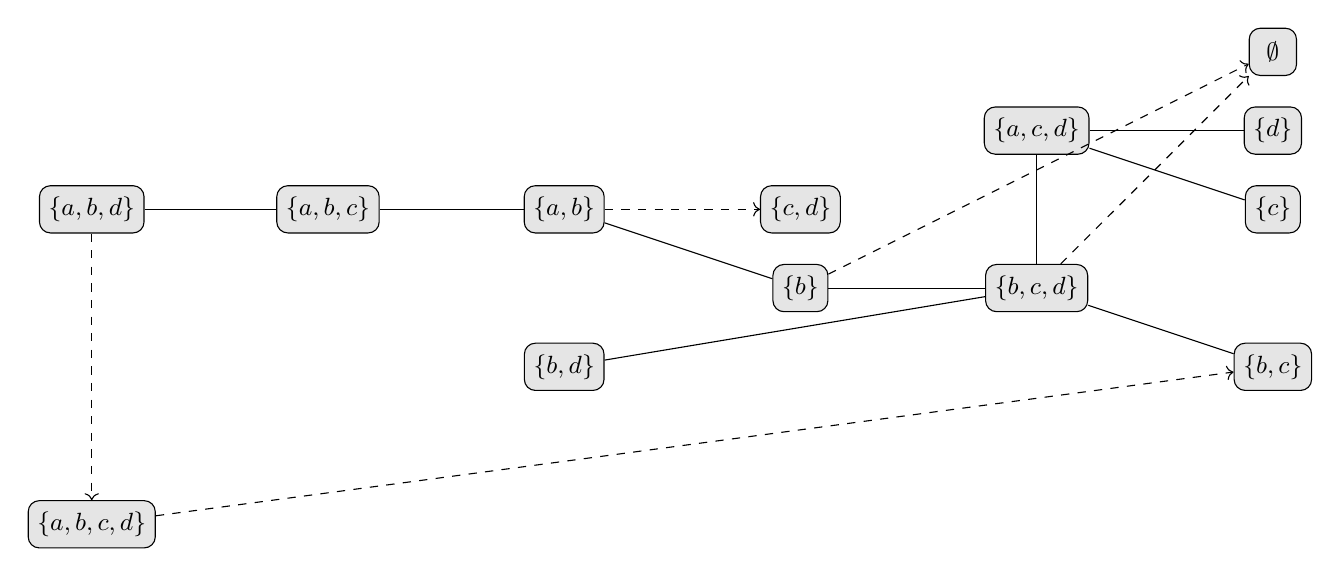
\begin{tikzpicture}[
    node distance=1.5cm and 2cm,
    every node/.style={
        draw,
        rectangle,
        rounded corners,
        fill=gray!20,
        minimum size=0.6cm,
        text centered,
        font=\small
    },
    every path/.style={
        draw,
        -{Stealth[scale=1]}
    }
]

% Define nodes
\node (A) at (0,0) {$\{a,b,d\}$};
\node (B) at (3,0) {$\{a,b,c\}$};
\node (C) at (6,0) {$\{a,b\}$};
\node (D) at (9,-1) {$\{b\}$};
\node (E) at (6,-2) {$\{b,d\}$};
\node (F) at (9,0) {$\{c,d\}$};
\node (G) at (12,1) {$\{a,c,d\}$};
\node (H) at (12,-1) {$\{b,c,d\}$};
\node (I) at (15,2) {$\emptyset$};
\node (J) at (15,1) {$\{d\}$};
\node (K) at (15,0) {$\{c\}$};
\node (L) at (15,-2) {$\{b,c\}$};
\node (M) at (0,-4) {$\{a,b,c,d\}$};

% Draw edges
\draw[-] (A) -- (B); % Solid arrow from {a,b,d} to {a,b,c}
\draw[-] (B) -- (C); % Solid arrow from {a,b,c} to {a,b}
\draw[-] (C) -- (D); % Solid arrow from {a,b} to {b}
\draw[-] (E) -- (H); % Solid arrow from {b,d} to {c,d}
\draw[-] (H) -- (G); % Solid arrow from {c,d} to {a,c,d}
\draw[-] (G) -- (J); % Solid arrow from {a,c,d} to {d}
\draw[-] (G) -- (K); % Solid arrow from {a,c,d} to {c}
\draw[-] (H) -- (L); % Solid arrow from {b,c,d} to {b,c}
\draw[-] (D) -- (H); % Solid arrow from {b} to {c,d}
\draw[dashed,->] (C) -- (F); % Dashed arrow from {a,b} to {c,d}
\draw[dashed,->] (D) -- (I); % Dashed arrow from {b} to \emptyset
\draw[dashed,->] (A) -- (M); % Dashed arrow from {a,b,d} to {a,b,c,d}
\draw[dashed,->] (M) -- (L); % Dashed arrow from {a,b,c,d} to {b,c}
\draw[dashed,->] (H) -- (I); % Dashed arrow from {c,d} to \emptyset

\end{tikzpicture}

\end{document}